\section{Zielsetzung}
In diesem Versuch werden die quantemechanischen Zustände zweier Rubidium Isotope (\ce{^{85}Rb}, \ce{^{87}Rb}) mittels optischen Pumpens untersucht. 
Dank der Zeemann-Aufspaltung der Energieniveaus durch ein externes Magnetfeld können die Landé-Faktoren und 
somit auch die Kernspins der Rubidium Isotope ermittelt werden.
Des Weiteren wird das Phänomen der Rabi-Oszillationen untersucht.

\section{Theorie}
\label{sec:Theorie}
Ähnlich wie beim Wasserstoffatom lassen sich auch die Energieniveaus des Valenzelektrons eines Alkalimetalls mit dem quantemechanischen Schalenmodell beschreiben.
Die verschiedenen Niveaus werden dabei über die Hauptquantenzahl $n \in \mathbb{N}$, die Bahndrehimpulsquantenzahl $L \leq n$, die 
magnetische Quantenzahl $m$ mit $-L \leq m \leq L$ und die Spinquantenzahl $S$ charakterisiert. 
Bei den vorliegenden Rubidium Isotopen gilt für den Grundzustand $L = 0$ und $S = \frac{1}{2}$. Der erste angeregte Zustand hat $L = 1$.
Ebenso wird der Kernspin über eine Quantenzahl $I$ mit Werten $I_{\ce{^{85}Rb}} = \frac{5}{2}$ und $I_{\ce{^{87}Rb}} = \frac{3}{2}$ beschrieben.

\subsection{Fein- und Hyperfeinstruktur}
Bei genauerer Betrachtung gibt es jedoch Korrekturen, die zu einer Aufspaltung dieser Niveaus führen.
Im Ruhesystem des Elektrons, rotiert der geladene Kern um das Elektron. Diese bewegte Ladung induziert ein Magnetfeld, welches mit dem magnetischen Moment 
\begin{equation}
    \label{eqn:mu_J}
    \vec{\mu}_J = -g_J \mu_B \vec{J}
\end{equation}
des Elektrons wechselwirkt. Dabei ist $\vec{J} = \vec{L} + \vec{S}$ der Gesamtdrehimpuls mit $|L-S| \leq J \leq L+S$ und 
$\mu_\text{B} = \frac{e \hbar}{2m_e}$ das Bohrsche Magneton. Der Faktor
\begin{equation}
    \label{eqn:g_J}
    g_J = 1 + \frac{J(J+1)+S(S+1)-L(L+1)}{2J(J+1)}
\end{equation}
wird Landé-Faktor genannt.
Aus diesem Grund werden die Energieniveaus des Elektrons in der Notation $n\ce{^{2S+1}L_J}$ angegeben, wobei $L$ ein Buchstabe ist, der den Bahndrehimpuls 
angibt (S: $L = 0$, P: $L = 1$). \\
Analog dazu, führt auch das magnetische Moment des Kerns zu einer Hyperfeinstruktur-Aufspaltung, die über die Quantenzahl $F$, mit $|J - I| \leq F \leq J + I$,
beschrieben wird.

\subsection{Zeemann-Effekt}
Eine weitere Aufspaltung kann durch das Anlegen eines externen Magnetfeldes erreicht werden. Hierbei koppelt erneut das magnetische Moment des Kerns
an das Magnetfeld, was zu einer Aufspaltung in $2F +1$ Energieniveaus mit Quantenzahlen $m_F$ ($-F \leq m_F \leq F$) führt. Der Abstand der Energieniveaus ist
dann durch 
\begin{equation}
    \label{eqn:E_Zeemann}
    \symup{\Delta}E_\text{Z} = g_F \mu_\text{B} B 
\end{equation}
gegeben, wobei $B$ die magnetische Flussdichte ist.
Der Landé-Faktor $g_F$ kann gemäß
\begin{equation}
              \label{eqn:g_F}
              g_F = g_J \frac{F(F+1)+J(J+1)-I(I+1)}{2F(F+1)}
\end{equation}
berechnet werden. \\
Die gesamte Aufspaltung der Zustände ist für die beiden Isotope \ce{^{85}Rb} und \ce{^{87}Rb} in \autoref{fig:rubidium_energy} gegeben. 
Der Grundzustand ist dabei das $5\ce{^{2}\text{S}_{\frac{1}{2}}}$-Orbital und der erste angeregte Zustand das $5\ce{^{2}\text{P}_{\frac{1}{2}}}$-Orbital.

\begin{figure}
    \centering
    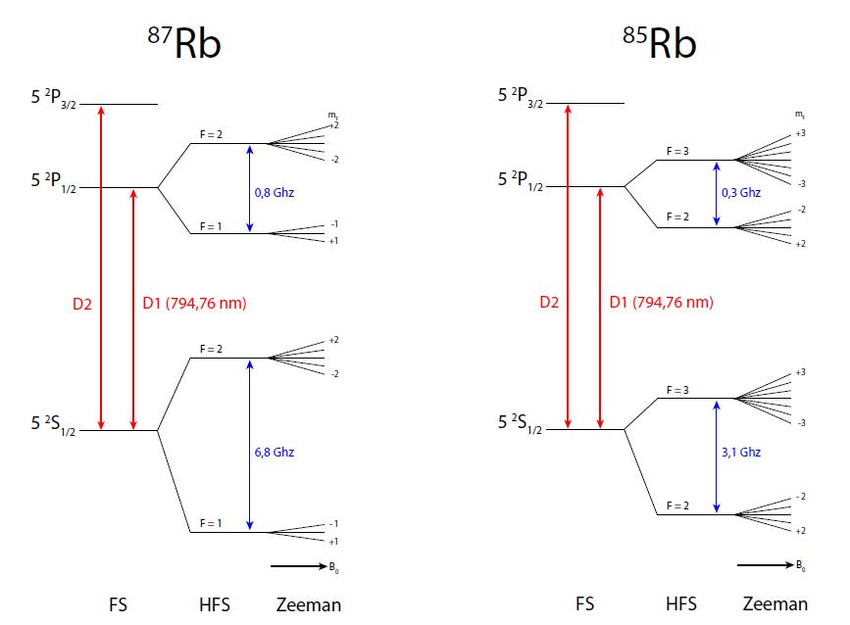
\includegraphics[width = \textwidth]{"content/pics/Rubidium_energy_levels.png"}
    \caption{Die Feinstruktur-, Hyperfeinstruktur- und Zeemann-Aufspaltung bei Rubidium \cite{Rubidium_energy}.}
    \label{fig:rubidium_energy}
\end{figure}

\subsection{Optisches Pumpen}
Bei Raumtemperatur folgt die Besetzung der Energieniveaus der Boltzmann-Statistik. Vor allem die verschiedenen Unterniveaus des Grundzustands 
($5\ce{^{2}\text{S}_{\frac{1}{2}}}$) sind besetzt. Durch einfallendes Licht können die Elektronen jedoch in höhere Zustände gehoben werden, wenn 
die Energie $E = hf$ des Photons genau der Energiedifferenz zweier Zustände entspricht. Beim optischen Pumpen wird dieser Effekt genutzt, um eine 
Besetzunginversion zu erzeugen, d.h. die Elektronen in höhere Zustände zu pumpen.
Ein Elektron, welches sich auf einem höheren Zustand befindet, kann entweder spontan oder durch stimulierte (induzierte) Emission ein Photon aussenden und 
wieder in einen energetisch niedrigeren Zustand zurück fallen. Bei stimulierter Emission wird durch ein einfallendes Photon ein Übergang des Elektrons
ausgelöst, bei welchem ein weiteres Photon gleicher Wellenlänge, Phasenlage und Polarisation emittiert wird.
Die spontane Emission folgt dabei einer $f^3$ Abhängigkeit und ist für die betrachteten Frequenzen 
deutlich wahrscheinlicher als die induzierte Emission, deren Wahrscheinlichekeit proportional zu $f$ ist. \\
In diesem Versuch wird $\text{D}1$-Licht verwendet, das Übergänge zwischen den $5\ce{^{2}\text{S}_{\frac{1}{2}}}$- und 
$5\ce{^{2}\text{P}_{\frac{1}{2}}}$-Niveaus anregt. Aus den Auswahlregeln für diese Übergänge folgt für linear polarisiertes Licht $\symup{\Delta}m_F = 0$
($\symup{\pi}$ Übergang) und für rechts- bzw. linkszirkular polarisiertes Licht $\symup{\Delta}m_F = +1$ ($\sigma^+$) und $\symup{\Delta}m_F = -1$ ($\sigma^-$).
Wird nun rechtszirkular polarisiertes $\text{D}1$-Licht eingestrahlt, werden die Elektronen aus dem $5\ce{^{2}\text{S}_{\frac{1}{2}}}$- in das 
$5\ce{^{2}\text{P}_{\frac{1}{2}}}$-Niveaus gehoben, wobei immer  $\symup{\Delta}m_F = +1$ gelten muss. Im angeregten Zustand fällt das Elektron nach gewisser
Zeit wieder in den Grundzustand zurück, wobei jedes Unterniveau gleich wahrscheinlich ist. Da allerdings für $m_F = 2$ keine erneute Anregung durch rechtszirkular
polarisiertes $\text{D}1$-Licht möglich ist ($\symup{\Delta}m_F = +1$), sammeln sich die Elektronen in diesem Niveau an. Dieser Zustand wird Besetzunginversion genannt.
Da nun keine weiteren Elektronen angeregt werden können, ist die Transmission des Lichtes maximal. \\
Ein Bruch dieser Besetzunginversion kann erreicht werden, wenn durch stimulierte Emission Übergänge zwischen den Unterniveaus innerhalb der 
$5\ce{^{2}\text{S}_{\frac{1}{2}}}$-Schale ausgelöst werden. Dies ist genau der Fall, wenn die Frequenz des RF-Magnetfeldes (Hochfrequenz) genau der 
Energiedifferenz der Unterniveaus entspricht. 
\begin{figure}
    \centering
    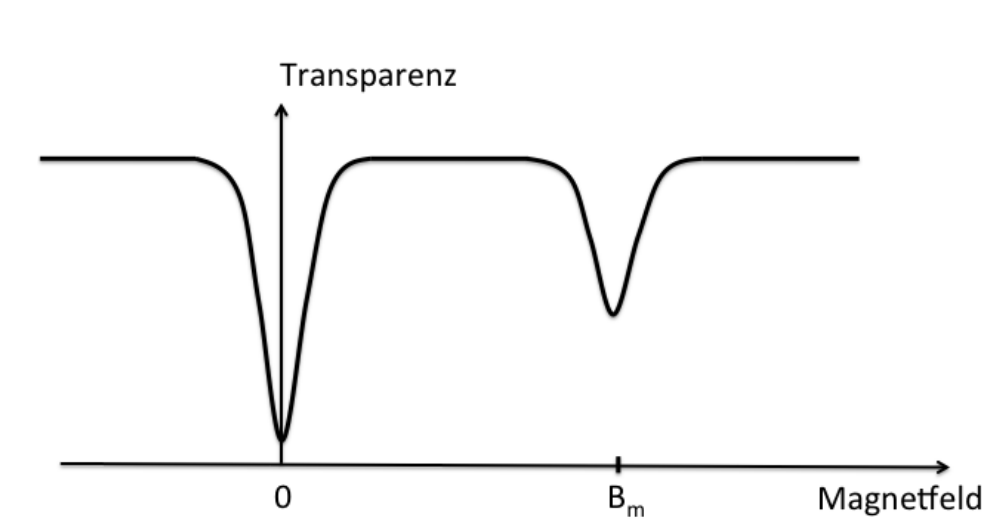
\includegraphics[width = .75\textwidth]{"content/pics/Messkurve_Theorie.png"}
    \caption{Transparenz einer Alkali-Dampfzelle für rechtszirkular-polarisiertes Licht in
    Abhängigkeit vom Magnetfeld der Sweep-Spule bei angelegten Hochfrequenzfeld
    (idealisierte Kurve) \cite{v21old}.}
    \label{fig:Mess_Theorie}
\end{figure}
Da die Zeemann-Aufspaltung proportional zu $B$ ist gilt dann nach \autoref{eqn:E_Zeemann} bei fester Frequenz
\begin{equation}
    \label{eqn:B_m}
    hf = g_F \mu_\text{B} B_m
\end{equation}
für den Betrag des Magnetfeldes $B_m$, bei dem die Besetzunginversion gebrochen wird.
Durch Auftragen der Transmission gegen $B$ unter Variation der Magnetfeldstärke lässt sich $B_m$ identifizieren und schließlich der Landé-Faktor $g_F$ bestimmen.
Die zu erwartende Messkurve ist in \autoref{fig:Mess_Theorie} dargestellt. Bei $B=0$ liegt keine Zeemann-Aufspaltung vor, weshalb die Transmission dort minimal ist.
An der Stelle $B_m$ gilt \autoref{eqn:B_m}. Da zwei verschiedene Isotope mit verschiedenen Landé-Faktoren vorliegen, werden zwei Einbrüche der Transmission nach 
$B = 0$ erwartet.

\subsection{Rabi-Oszillationen}
Durch schnelles Ein- und Ausschalten des RF Feldes an der Resonanzstelle $B_m$ beginnt der Spin $\vec{F}$ um die Richtung des äußeren Magnetfeldes zu 
präzidieren. Die Frequenz der Präzession wird Lamorfrequenz genannt und berechnet sich zu $\omega = \gamma \cdot B$ mit dem gyromagnetischen Verhältnis 
$\gamma = g_F \sfrac{e}{2m_e}$. Dieser Effekt spiegelt sich in Oszillationen der Transmission (Rabi-Oszillationen) wieder. Mit der Periodendauer $T$ lässt sich 
das Verhältnis
\begin{equation}
    \frac{T_{\ce{^{85}Rb}}}{T_{\ce{^{87}Rb}}} = \frac{\gamma_{\ce{^{87}Rb}}}{\gamma_{\ce{^{85}Rb}}} = \frac{g_{F \;{\ce{^{87}Rb}}}}{g_{F \;{\ce{^{85}Rb}}}}
\end{equation}
aufstellen.
Der Anstieg der Transmission beim Ausschalten des Magnetfeldes folgt einem Exponentialgesetz.
